\documentclass{beamer}

\usepackage[frenchb]{babel}
\usepackage{graphicx}
\usepackage[utf8]{inputenc} % Required for inputting international characters
\usepackage[T1]{fontenc} % Output font encoding for international characters
\usepackage{listings}
\usepackage{xcolor}
\usepackage{bbm}
\usepackage{amsmath}
\usepackage{amsfonts}
\usepackage{amssymb}
\usepackage{eqnarray}
\usepackage{hyperref}
\usepackage{url}

\mode<presentation>
{
 \usetheme{Warsaw}
}

\setbeamertemplate{footline}
{
  \leavevmode%
  \hbox{%
  \begin{beamercolorbox}[wd=.5\paperwidth,ht=2.25ex,dp=1ex,center]{author in head/foot}%
    \usebeamerfont{author in head/foot}{Mohammed Amine KHELDOUNI}
  \end{beamercolorbox}%
  \begin{beamercolorbox}[wd=.5\paperwidth,ht=2.25ex,dp=1ex,center]{title in head/foot}%
    \usebeamerfont{title in head/foot}\insertshorttitle\hspace*{3em}
    \insertframenumber{} / \inserttotalframenumber\hspace*{1ex}
  \end{beamercolorbox}}%
  \vskip 0pt%
}

%----------------------------------------------------------------------------------------
%	TITLE PAGE
%----------------------------------------------------------------------------------------

\title[Projet MOPSI]{Calibration en finance - Mélange de Black-Scholes} % The short title appears at the bottom of every slide, the full title is only on the title page
\author{Mohammed Amine KHELDOUNI} % Your name
\institute[ENPC] % Your institution as it will appear on the bottom of every slide, may be shorthand to save space
{Ecole des Ponts ParisTech \\ % Your institution for the title page
\medskip
}
\date{\today} % Date, can be changed to a custom date


% Progressbar
\usepackage{tikz}
\usetikzlibrary{calc}

\makeatletter
\def\progressbar@progressbar{} % the progress bar
\newcount\progressbar@tmpcounta% auxiliary counter
\newcount\progressbar@tmpcountb% auxiliary counter
\newdimen\progressbar@pbht %progressbar height
\newdimen\progressbar@pbwd %progressbar width
\newdimen\progressbar@tmpdim % auxiliary dimension

\progressbar@pbwd=\paperwidth
\progressbar@pbht=1pt

\def\progressbar@progressbar{%

\progressbar@tmpcounta=\insertframenumber
\progressbar@tmpcountb=\inserttotalframenumber
\progressbar@tmpdim=\progressbar@pbwd
\multiply\progressbar@tmpdim by \progressbar@tmpcounta
\divide\progressbar@tmpdim by \progressbar@tmpcountb

  \begin{tikzpicture}[very thin]

  \shade[draw=red,top color=red!10,bottom color=red!10,middle color=red] %
    (0pt, 0pt) rectangle ++ (\progressbar@tmpdim, \progressbar@pbht);

  \end{tikzpicture}%
 }

\addtobeamertemplate{frametitle}{}
{%
 \vspace*{-20pt}
  \begin{beamercolorbox}[wd=\paperwidth,ht=1pt,dp=1pt]{}%
    \progressbar@progressbar%
  \end{beamercolorbox}%
}%
\makeatother

\begin{document}

\AtBeginSection[]{\frame{\sectionpage}}

\begin{frame}
\titlepage % Print the title page as the first slide
\end{frame}

\begin{frame}\frametitle{Plan}
\tableofcontents
\end{frame}

\section{Présentation du problème}
\subsection{Définition des paramètres}

\begin{frame}
On veut connaître le prix d'une action sur le marché. Une \textit{action} est un titre de propriété délivré par une société de capitaux.
\textbf{Paramètres :}
\begin{itemize}
  \item $T$ : La maturité désigne le temps qui sépare la date à laquelle une obligation est émise, et la date à laquelle la valeur nominale de cette obligation est remboursée.
  \item une option :  Produit dérivé qui établit un contrat entre un acheteur et un vendeur.
  \item $S_t$ : Un actif sous-jacent est un actif sur lequel porte une option ou plus largement un produit dérivé.
  \item $r$ : Le taux d'intérêt fixe la rémunération du capital prêté versé par l'emprunteur au prêteur.
\end{itemize}
\end{frame}

\subsection{Description du modèle}

\begin{frame}
  \vspace{1cm}
    \begin{itemize}
      \item $\sigma$ : La volatilité est l'ampleur des variations du cours d'un actif financier. Elle sert de paramètre de quantification du risque de rendement et de prix d'un actif financier. \newline Lorsque la volatilité est élevée, la possibilité de gain est plus importante, mais le risque de perte l'est aussi.
      \item $K$ : Le strike désigne le prix d'exercice d'une option, qui correspond au prix fixé dans le contrat pour l’acquisition ou la cession du sous-jacent.
    \end{itemize}
  \end{itemize}
\end{frame}


\begin{frame}
  \begin{itemize}
    \item Call : Le call ou l'option d'achat est une option d'achat sur un instrument financier.
    \item Put : A l'opposé du Call, le Put est l'option de vente de cet instrument.
  \end{itemize}
  Etant donné les paramètres $\sigma$, $T$, $K$, $S_0$ et $r$ on voudrait calculer le prix d'un call ou d'un put sur le marché, pour un actif financier.

\end{frame}

\section{Modélisation mathématique du marché}
\begin{frame}{Modèle de Black-Scholes}
  Dans ce modèle, on considére le prix de l'action comme un processus stochastique en temps continu $S_t$. \newline
  \textbf{Hypothèses :}
  \begin{itemize}
    \item  Marchés efficients :
    \begin{itemize}
      \item Pas de coûts de transaction
      \item Pas de restrictions sur le volume de transactions
      \item Pas d'opportunité d'arbitrage
    \end{itemize}
    \item Les rendements du sous-jacent sont gaussiens, stationnaires et indépendants.
    \item Le placement à la banque est sans risque et le taux d'intérêt r est constant.
  \end{itemize}
\end{frame}
\begin{frame}
  \textbf{Equation différentielle stochastique}
  $$ dS_t = \mu S_t dt + \sigma S_t dW_t $$
On note \begin{itemize}
      \item $S_0$ - La valeur actuelle de l'action sous-jacente.
      \item $T$ - Le temps qu'il reste à l'option avant son échéance (la maturité).
      \item $K$ - Le prix d'exercice fixé par l'option.
      \item $W_t$ - Mouvement Brownien de variance $t$
\end{itemize}
\end{frame}

\begin{frame}{Formule de Black-Scholes : Le Call}
Le prix théorique d'un call donnant le droit mais pas l'obligation d'acheter l'actif $S$ à la valeur $K$ à la date $T$, est caractérisé par son \textit{payoff}:
$$ (S_T - K)^{+} = \max (S_T -K,0) $$
La formule de Black-Scholes donne le prix d'un Call :
$$ C(S_0,K,r,t,\sigma) = S_0 \phi(d_1)-K \times e^{-rt} \phi(d_2) $$
Avec : \begin{itemize}
\item $\phi$ la fonction de répartition de la loi normale centrée réduite.
\item $d_1 = \frac{1}{\sigma \sqrt{t}} (ln(\frac{S_0}{K})+(r+\frac{1}{2}\sigma^2)t) $
\item $d_2 = d_1 - \sigma \sqrt{t}$
\end{itemize}
\end{frame}

\begin{frame}{Formule de Black-Scholes : Le Put}
Et pour un put, on a un prix théorique par rapport à un \textit{payoff} de $ (S_T - K)^{+}$
\\ \vspace{0.5cm}
Et on a une formule de Black-Scholes pour le prix d'un put :
$$ P(S_0,K,r,t,\sigma) = -S_0 \phi(-d_1)+K \times e^{-rt} \phi(-d_2) $$

\end{frame}

\begin{frame}{Mélange de modèles de Black-Scholes}
  On fixe un nombre $P$ de modèles de Black-Scholes dont on va effectuer un mélange selon une certaine distribution de probabilités $(p_1,p_2,...,p_p)$.
  \newline
  Ainsi on considère le Call (et on fait de même pour le prix d'un Put), à $K$, $r$ et $t$ fixés, de notre mélange comme suit :
  $$ C_m(\lambda, \sigma, p) = \sum^p_{i=1} p_i C(\lambda_i,K,r,t,\sigma_i) $$
\begin{itemize}
  \item $\lambda$ : la liste de taille $P$ des sous-jacents de chacun des modèles considérés.
  \item $\sigma$ : la liste des volatilités
  \item $p$ : la liste des probabilités de tirer chacun des modèles.
\end{itemize}
\end{frame}

\section{Optimisation des paramètres du marché}
\begin{frame}{Présentation du programme d'optimisation}
  En considérant un vecteur $ \beta_0 = (\lambda,\sigma,p)$ fixé, on obtient par la formule de Black-Scholes les prix d'un Call et d'un Put d'une option qu'on prend européenne par exemple.
  \newline
  En oubliant la valeur $\beta_0$, on peut la retrouver en effectuant une méthode des moindres carrés sur plusieurs prix d'exercice $(K_1,...,K_M)$, minimisant les résidus des prix. Pour un call :
  $$ \min \sum^M_{j=1} (C_{m,j}(\beta)-\alpha_j)^2 $$
  \vspace{-0.3cm}
  $$ s.c. \sum^p_{i=1}p_i = 1 $$
$\alpha_j$ étant le prix du Call calculé pour $\Beta_0$ pour un \textit{Strike} $K_j$.
\end{frame}

\begin{frame}{Résultats d'optimisation}
    \begin{minipage}{0.49\textwidth}
      On prend $P = 2$
      \begin{itemize}
        \item $\lambda = (100,100)$
        \item $\sigma = (0.2, 0.4)$
        \item $p = (0.5,0.5) $
        \item $r = 0$
        \item $K = (50,...150)$
      \end{itemize}
    \end{minipage}

    \begin{minipage}{1.49\textwidth}
    \begin{figure}[!r]
      \vspace{-3cm}
      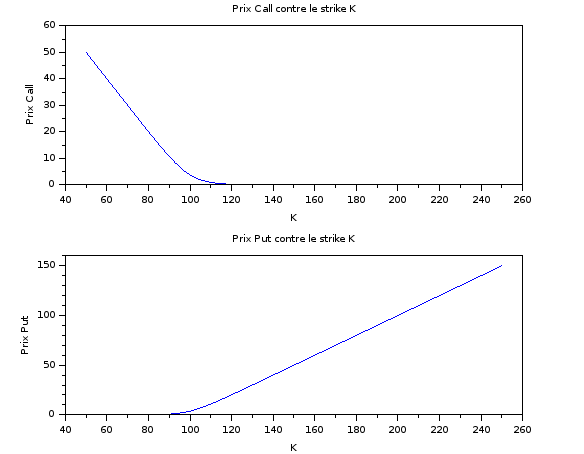
\includegraphics[scale=0.35]{callput.png}
    \end{figure}
    \end{minipage}
\end{frame}

\begin{frame}
  On trouve par la fonction d'optimisation non linéaire de SCILAB, \textit{optim}, un $\beta$ proche de l'optimum :
  $$ \beta_* = (100.001,100.001,0.22,0.38,0.5,0.5) $$
  Toutefois, les erreurs de calibrations étant non négligeables, il a fallu réajuster l'ensemble de recherche des solutions réalisables.
\end{frame}

\section{Problèmes de calibration}

\begin{frame}{Minimisation en grande dimension}
  En effet, même pour $p=2$, il a fallu ajuster un bon intervalle pour le strike $K$, pour que l'optimisation des moindres carrés donne un résultat cohérents avec le $\beta_0$ qu'on a "oublié" pour retrouver par cette méthode.
  \newline
  En augmentant la dimension de l'espace dans lequel vit $\beta$, de dimension $3P$, l'optimisation ne marche plus.
  $$ \Rightarrow \text{C'est un problème de calibration en finance} $$
\end{frame}

\section{Formule de Black-Scholes inversée}
\subsection{Explication du problème}

\begin{frame}{Explication de l'inversion de Black-Scholes}
Cette fois-ci, connaissant tous les paramètres sauf la volatilité $\sigma$, on va essayer de la retrouver pour un certain sous-jacent du marché. \newline
Sur le marché, on connait le dernier prix d'un Call/Put émis pour un actif financier et par la formule de Black-Scholes, on inverse l'équation.
\newline Donc :
$$ \exists ! \sigma_* s.t. \ \ \ C_{BS}(S_0,K,r,t,\sigma_*) = C_{market} $$
On appelle cette volatilité, la \textbf{volatilité implicite}.

\end{frame}

\subsection{Modèles de résolution}
\begin{frame}{Recherche de la volatilité implicite}
Il existe divers méthodes de résolution de l'inversion de la formule de Black-Scholes :
\begin{itemize}
  \item Méthode de Newton-Raphson de convergence quadratique
  \item La dichotomie de convergence en $\mathcal{O}(log(M))$
\end{itemize}
\end{frame}

\subsection{Résultats}


\begin{frame}{Résultats}
  En utilisant la fonction \textit{fsolve} de SCILAB, on obtient un graphe 3D appelé \textbf{la surface de la volatilité} pour les valeurs précédentes avec $M=200$ le nombre de prix d'exercices pris en compte.
    \begin{figure}
      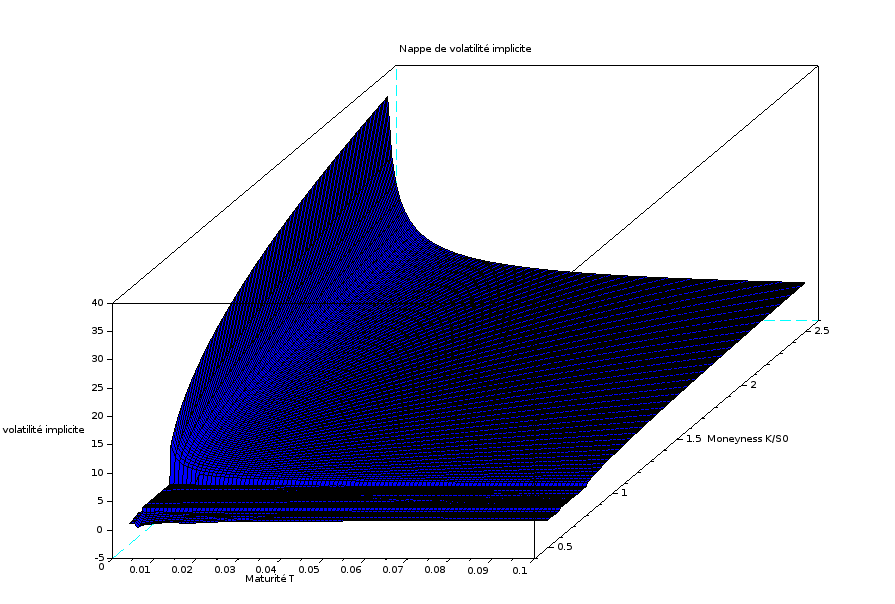
\includegraphics[scale=0.20]{volimpl1.png}
    \end{figure}
\end{frame}

\begin{frame}{Données de Google en 2008}
  On prend $M = 200$ et :

    \[
      \begin{array}{|c|c|}
        \hline
        S_0 & 505.15 \\ \hline
        \sigma_0 & 20\% \\ \hline
        r & 3.3 \% \\ \hline
        K & (500,...,700) \\ \hline
        T & 2 \\ \hline
      \end{array}
    \]
\end{frame}


\begin{frame}{Résultat}
    \begin{figure}
      \vspace{-0.8cm}
      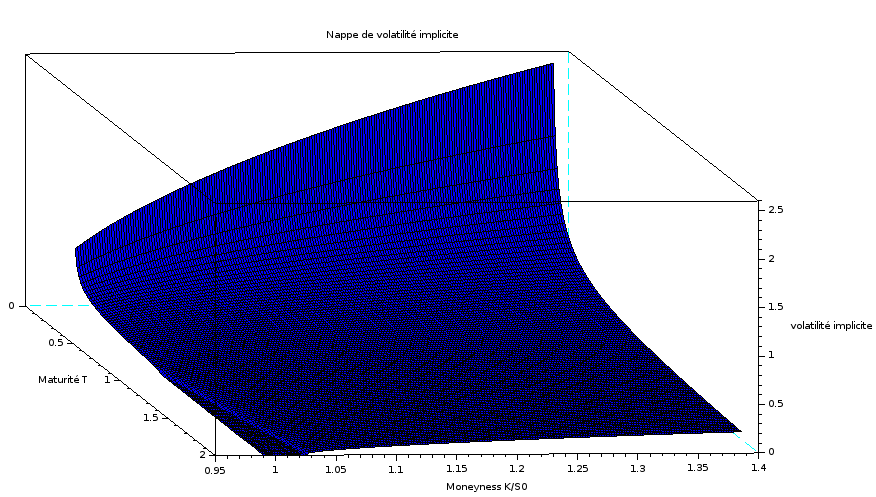
\includegraphics[scale=0.35]{volimpl2.png}
    \end{figure}
\end{frame}

\begin{frame}{Commentaires}
  On remarque bien un phénomène de lissage de la surface de volatilité tout au long de l'exercice de l'option et pour diverses valeurs de sa maturité $T$.
  \newline
  Néanmoins, il subsiste selon les paramètres d'entrée quelques irrégularités de la nappe dûes à une mauvaise approximation de la volatilité de l'actif. Il faut donc affiner la convergence par une dichotomie pour une méthode de Newton et comparer.
  \newline
  La volatilité baisse sur une grande échéance et atteint de plus grandes valeurs pour de grand taux de \textit{moneyness} ou de prix d'exercices $K$.
\end{frame}
\section{Applications : Prix du marché - Boursorama}
\subsection{Données}
\subsection{Anticipation sur le prix d'un actif}


\begin{frame}{Données}
\end{frame}

\begin{frame}{Anticipation sur le prix d'un actif}
\end{frame}

%\begin{frame}{Bibliographie}
%\begin{itemize}

%   \item \url{https://fr.wikipedia.org/wiki/Maturit%C3%A9_(finance)}
%   \item \url{https://fr.wikipedia.org/wiki/Action_(finance)}
%   \item \url{https://fr.wikipedia.org/wiki/Actif_sous-jacent}
%   \item \url{https://fr.wikipedia.org/wiki/Taux_d%27int%C3%A9r%C3%AAt}
%   \item \url{https://fr.wikipedia.org/wiki/Volatilit%C3%A9_(finance)}
%\end{itemize}
%\end{frame}

\end{document}
